% ***************************** MAIN FILE **********************************
\documentclass[12pt]{report}           % Art des zu erstellenden Dokuments
% bei zweiseitigem Druck twoside-Option oder book-Klasse verwenden

% ****************************** PREAMBLE **********************************
% **************************** PACKAGE SETUP *******************************
\usepackage[ngerman]{babel}          % Lokalisierung von Typographie, Silbentrennung, etc.

\usepackage{ucs}                     % Erweiterte Unterstützung von UTF-8-Kodierung
\usepackage[utf8x]{inputenc}         % Unterstützung von UTF-8 in Eingabe-Dateien
\usepackage[T1]{fontenc}             % Zeichensatzkodierung von LaTeX (Cork-Kodierung)
\usepackage{textcomp}				 % Text-Companion-Symbols (z. B. \texteuro)
\usepackage{ae}						 % Schöne Schriften für PDF-Dateien
\usepackage{helvet,courier,mathptmx} % Verwendete Schriftarten

\usepackage{amsmath}                 % Mathematische Infrastruktur für LaTeX der AMS
\usepackage{amsfonts}                % Mathematische Schriftarten
\usepackage{amssymb}                 % Mathematische Symbole
\usepackage{amsthm}                  % Erweiterung der Theorem-Umgebungen

\usepackage[ngerman]{translator}
%Paket laden
\usepackage[
%xindy,
%nonumberlist, %keine Seitenzahlen anzeigen
nopostdot,    %Den Punkt am Ende jeder Beschreibung deaktivieren
acronym,      %ein Abkürzungsverzeichnis erstellen
%toc
]      %im Inhaltsverzeichnis auf section-Ebene erscheinen
{glossaries}


\usepackage{fancyhdr}                % Erweiterte Konfiguration von Kopf/Fußzeile
\usepackage{hyperref}                % Querverweise, Hyperlink, pdf-Konfiguration, etc.

\usepackage{float}                   % Selbstdefinierte Floating-Umbgebungen
\usepackage{tabularx}                % Tabellen mit einstellbarer Spaltenbreite
\usepackage{colortbl}                % Für Farben in Tabellen
\usepackage[labelfont=bf]{caption}   % Anpassen der Abbildungs- und Tabellenbeschriftungen

\usepackage{algpseudocode}           % Algorithmen als Pseudocode (basiert auf algorithmicx)
\usepackage{listings}                % Quellcode-Satz (z.B. mit Syntax-Hervorhebung)

\usepackage{graphicx}                % Erweiterte Unterstützung von Graphiken
\usepackage{textpos}                 % Beliebig platzierte Textboxen
\usepackage{xcolor}                  % TeX-Engine-unabhängige Definition von Farben

\usepackage[numbers]{natbib}         % Weiter Optionen für die Bibliographie

\usepackage{setspace}
\usepackage{ellipsis}	% Korrigiert den Wei�raum um Auslassungspunkte
\usepackage{placeins} 
\usepackage{tikz}
\usepackage{pifont}                  % Zum Benutzen der pifont Commands for Using Zapf Dingbats Symbole

% ****************************** TOP MATTER ***********************************
\renewcommand{\author}{Stefan Kruk}           % Name
\newcommand{\dateOfBirth}{14.08.1992}           % Geburtsdatum
\newcommand{\matrNumber}{xxxxxxx}              % Matrikelnummer
\newcommand{\studycourse}{Softwaretechnik (Dual)}           % Studiengang

\newcommand{\supervisor}{Dr. Kim Lauenroth} % Betreuer
\newcommand{\institution}{Fachhochschule Dortmund} % Hochschule
\newcommand{\faculty}{Informatik}               % Fachbereich
\newcommand{\toponym}{Dortmund}                 % Ort

\newcommand{\subject}{Seminararbeit}  % Art/Thema der Arbeit
\newcommand{\titel}{Continuous Delivery} % Titel der Arbeit
%\newcommand{\subtitel}{Zweizeiliger Untertitel\\sofern vorhanden} % Untertitel
%\newcommand{\degree}{Bachelor/Master of Art} % Angestrebter Titel (nur bei Abschlussarbeiten, sonst leer lassen/auskommentieren)

\newcommand{\keywords}{Vorlage, Seminararbeit, Continuous Delivery, Informatik, {FH Dortmund}} % Stichworte (durch Komma getrennt)

% **************************** HYPERREF SETUP *******************************
\definecolor{linkcolor}{rgb}{1,0.5,0}
\hypersetup
{
bookmarks=true,                        % Lesezeichen im PDF erzeugen
bookmarksopen=true,                    % Lesezeichen im PDF sofort anzeigen
backref=true,                          % Rückverweise im Literaturverzeichnis
colorlinks=true,                       % Farbige Verweise
%hidelinks = true,                      % Verweise verbergen (entfernt Farbe und Rahmen)
pdfstartview={FitH},                   % Ansicht des PDFs beim öffnen
pdftitle={\titel},                     % Title des PDFs
pdfauthor={\author , \supervisor},     % Autor des PDFs
pdfsubject={\subject},                 % Thema des PDFs
%pdfcreator={Creator},                 % Erzeuger des Dokuments (Anwendungsprogramm)
%pdfproducer={Producer},               % Ersteller des PDFs (Programm/Bibliothek/Skript)
pdfkeywords={\keywords},               % Stichwörter zum PDF
linkcolor=linkcolor,                   % Farbe von Querverweisen
citecolor=linkcolor,                       % Farbe von Zitaten
filecolor=magenta,                     % Farbe von Verweisen auf Dateien
urlcolor=cyan                          % Farbe von URLs
}
% Weitere Optionen: http://www.tug.org/applications/hyperref/manual.html

% Für Zeichnungen
\usetikzlibrary{% 
    arrows,% 
    calc,% 
    fit,% 
    patterns,% 
    plotmarks,% 
    shapes.geometric,% 
    shapes.misc,% 
    shapes.symbols,% 
    shapes.arrows,% 
    shapes.callouts,% 
    shapes.multipart,% 
    shapes.gates.logic.US,% 
    shapes.gates.logic.IEC,% 
    er,% 
    automata,% 
    backgrounds,% 
    chains,% 
    topaths,% 
    trees,% 
    petri,% 
    mindmap,% 
    matrix,% 
    calendar,% 
    folding,% 
    fadings,% 
    through,% 
    positioning,% 
    scopes,% 
    decorations.fractals,% 
    decorations.shapes,% 
    decorations.text,% 
    decorations.pathmorphing,% 
    decorations.pathreplacing,% 
    decorations.footprints,% 
    decorations.markings,% 
    shadows
} 

% **************************** LISTINGS SETUP *******************************
\definecolor{keywords}{rgb}{0.5 0 0.3}
\definecolor{comments}{rgb}{0.25,0.5,0.37}
\definecolor{lila}{RGB}{112, 6, 147}
\definecolor{kommentgreen}{RGB}{5,132,71}
\definecolor{grey}{RGB}{242,242,242}  
\definecolor{darkgreen}{named}{green}
\definecolor{darkblue}{named}{blue}
\definecolor{lightblue}{RGB} {63,95,191}
\definecolor{darkred}{named}{red}
\definecolor{grau}{named}{gray}
\definecolor{fh_orange}{rgb}{0.953,0.201,0}
\definecolor{fh_grau}{rgb}{0.76,0.75,0.76}

\definecolor{listinggray}{gray}{0.9}
\definecolor{lbcolor}{rgb}{0.9,0.9,0.9}
\lstset{literate=%
    {Ö}{{\"O}}1
    {Ä}{{\"A}}1
    {Ü}{{\"U}}1
    {ß}{{\ss}}1
    {ü}{{\"u}}1
    {ä}{{\"a}}1
    {ö}{{\"o}}1
    {~}{{\textasciitilde}}1
}
\lstset{ %
    backgroundcolor=\color{grey},   % Hintergrundfarbe
    basicstyle=\linespread{0.94}\footnotesize\ttfamily, % Schrifteinstellungen für Quellcode
    breakatwhitespace=false,         % Automatische Zeilenumbrüche nur bei Leer- oder Tabulatorzeichen (Leerraum/whitespaces)
    breaklines=true,                 % Automatische Zeilenumbrüche
    captionpos=b,                    % Beschriftung unten
    commentstyle=\color{comments},   % Schrifteinstellungen für Kommentare
    columns=felxible,                 % Ist notwendig, damit man Quellcode aus den Listings kopieren kann
    %  deletekeywords={...},            % Bestimmte Schlüsselwörter entfernen
    escapeinside={\%*}{*)},          % Defintion von Escape-Sequenzen
    extendedchars=false,                   % Nicht ASCII-Zeichen erlauben
    frame=single,                    % Rahmen um den Quellcode
    keepspaces=true,                 % Einrückungen im Quellcode behalten
    keywordstyle=\bfseries\color{keywords},% Schrifteinstellungen für Schlüsselwörter
    language=java,                   % Programmiersprache des Quellcodes
    %  morekeywords={*,...},            % Zusätzliche Schlüsselwörter
    numbers=left,                    % Zeilennummerierung
    numbersep=5pt,                   % Abstand zwischen Zeilennummerierung und Quellcode
    numberstyle=\color{black}, % Schrifteinstellungen für Zeilennummern
    rulecolor=\color{black},         % if not set, the frame-color may be changed on line-breaks within not-black text (e.g. comments (green here))
    showspaces=false,                % Leerraum-Zeichen anzeigen
    showstringspaces=false,          % Leerzeichen in Zeichenketten anzeigen
    showtabs=false,                  % Tabulatorzeichen in Zeichenketten anzeigen
    stepnumber=1,                    % Schrittweite bei Zeilennummern
    stringstyle=\color{blue},        % Schrifteinstellungen für Zeichenketten
    tabsize=4,                       % Tabulatorbreite (Anzahl Leerzeichen)
    numberbychapter=false            % Nummeriere Quellcode fortlaufend je Kapitel
}

\lstdefinestyle{java}
{
    language=Java,
    keywordstyle=\bfseries\color{lila},  	% underlined bold black keywords 
    identifierstyle=\bfseries\color{blue}, 
    commentstyle=\bfseries\color{kommentgreen}, % white comments 
    stringstyle=\bfseries\color{black},
}

\lstdefinestyle{xml}
{
    language=xml,
    basicstyle=\fontsize{9pt}{9pt}\selectfont\color{kommentgreen},
    keywordstyle=\color{lila},  	% underlined bold black keywords 
    %Hier können bei Bedarf noch weitere Keywords eingetragen werden
    keywords={name, value, version, encoding, id, type, xmlns:xsi, ref, namespace},
    identifierstyle=\color{black},  
    stringstyle=\color{blue},  
    commentstyle=\color{lightblue},
    morecomment=[s]{<!--}{-->},
    rulecolor=\color{black}
}
\renewcommand{\lstlistlistingname}{Quellcodeverzeichnis}
\renewcommand{\lstlistingname}{Quellcode}

\AtBeginDocument{\numberwithin{lstlisting}{section}} % Nummeriere Quellcode fortlaufend je Abschnitt

% ************************** HEADER/FOOTER SETUP ****************************
\setlength{\headheight}{15pt}

\renewcommand{\chaptermark}[1]{ \markboth{#1}{} }

\fancyhf{}
\fancyhead[LE]{\thepage \ \ \ \ {\tiny \author, \today}}
\fancyhead[RO]{{\tiny \author, \today} \ \ \ \ \thepage}
\fancyhead[LO,RE]{\textit{\nouppercase{\leftmark}} }
\renewcommand{\headrulewidth}{0pt}

% **************************** GRAPHICX SETUP *********************************
\DeclareGraphicsExtensions{.pdf,.png,.jpg} % bekannte Graphik-Dateiformate (müssen nicht mehr im Dateinamen angegeben werden, also statt "beispiel.png" nur noch "beispiel")
\graphicspath{{./figure/}}   % path to graphics folder, usage {PATH},{ANOTHERPATH}...

% ************************** BIBLIOGRAPHY SETUP ********************************
\bibliographystyle{dinat}    % Literaturverzeichnis nach DIN
%\AtBeginDocument{\nocite{*}} % Diese Zeile vor der Abgabe der Arbeit entfernen!

% ****************************** MATH SETUP ************************************
\everymath{\displaystyle}    % Erzwinge \displaystyle für Mathematischen-Modus


% ************************* THEOREMS AND PROOF *********************************
\newtheoremstyle{thesis}     % Name des neuen Theorem-Stils
{3pt}                        % Abstand oberhalb des Theorems
{3pt}                        % Abstand unterhalb des Theorems
{\itshape}                   % Schrifteinstellungen innerhalb des Theorems
{}                           % Einrückung der Theorem-Überschrift
{\bfseries}                  % Schrifteinstellungen für die Überschrift des Theorems
{}                           % Satzzeichen zwischen Überschrift und Theorem-Rumpf
{\newline}                   % Abstand hinter der Überschrift
{}                           % Spezifikation der Überschrift
  
\theoremstyle{thesis}        % Verwende neuen Theorem-Stil

\newtheorem{theorem}{Satz}[section] % neue Theorem-Umgebung: theorem (Satz)
\providecommand*{\theoremautorefname}{Satz} % autoref-Name für theorem

\newtheorem{definition}{Definition}[section] % neue Theorem-Umgebung: definition (Definition)
\providecommand*{\definitionautorefname}{Definition} % autoref-Name für definition

\renewcommand{\qedsymbol}{$\blacksquare$} % Schwarzes Quardrat als Symbol für: q. e. d.
\renewenvironment{proof}[1][\proofname]{{\bfseries #1:}~}{\qed} % "Beweise:" in Fettdruck

% *************************** PSEUDOCODE SETUP ********************************
\floatstyle{boxed}                        % Rahmen für pseudocode-Umgebung
\newfloat{pseudocode}{htbp}{lop}[section] % Definieren pseudocode-Umgebung
\floatname{pseudocode}{Pseudocode}        % Beschrifte pseudocode-Umgebung mit "Pseudocode"

\newcommand{\listofpseudocodename}{Pseudocodeverzeichnis}
\newcommand{\listofpseudocode}{\listof{pseudocode}{\listofpseudocodename}}
\providecommand*{\pseudocodeautorefname}{Pseudocode}

% ******************************* PAGE SETUP **********************************
\textheight23cm
\textwidth14cm
\voffset0cm
\topskip0cm
\topmargin-1.2cm
\headheight1.0cm
\headsep1.5cm
\oddsidemargin1.0cm
\evensidemargin1.0cm
\renewcommand{\baselinestretch}{1.4} 
\widowpenalty=300
\clubpenalty=300

% ******************************** MACROS *************************************
\newcommand{\RR}{\mathbf{R}}
\newcommand{\NN}{\mathbf{N}}
\newcommand{\QQ}{\mathbf{Q}}
\newcommand{\ZZ}{\mathbf{Z}}
\newcommand{\CC}{\mathbf{C}}
\newcommand{\quelle}{\footnotesize Quelle: }

\newcommand{\suchstring}[1]{$S_{#1}$}
\newcommand{\suchstringPrefix}{("'Continuous Delivery"` OR "'Deployment"`)}

\newcommand{\greenchecked}{\textcolor{green}{\textbf{\ding{52}}}}
\newcommand{\redX}{\textcolor{red}{\textbf{\ding{56}}}}

\newcolumntype{L}[1]{>{\raggedright\arraybackslash}p{#1}} % linksbündig mit Breitenangabe
\newcolumntype{C}[1]{>{\centering\arraybackslash}p{#1}} % zentriert mit Breitenangabe
\newcolumntype{R}[1]{>{\raggedleft\arraybackslash}p{#1}} % rechtsbündig mit Breitenangabe

%Befehle für Glossar
\newglossaryentry{glos:TTM}{
    name=Time-to-Market,
    description={Unter dem Begriff Time-to-Market wird die Zeit von der Produktentwicklung bis zur Auslieferung auf dem Markt verstanden. In dieser Zeit müssen Kosten für die Erstellung/Entwicklung aufgebracht werden, es spielt aber keine Umsätze ein. Daher strebt jedes Unternehmen eine möglichst geringe Time-to-Market Zeit an. Insbesondere wenn es um Wettbewerb geht, muss diese Zeit kurz gehalten werden.}
}

%%%%%%%%%%%%%%%%%%%%%%%%%%%%%%%%%%%%%%%%%%%%%%%%%%%%%%%%%%%%%%%%%%%%%%%%%%%%%%%
% ************************** BEGINN OF DOCUMENT *******************************
%%%%%%%%%%%%%%%%%%%%%%%%%%%%%%%%%%%%%%%%%%%%%%%%%%%%%%%%%%%%%%%%%%%%%%%%%%%%%%%
\begin{document}

\begin{titlepage}
%FH LOGO
% \includegraphics[width=3.8cm]{content/images/logo}

% *** Subject ***
{\centering {\Huge \bfseries \subject\par}}
% *** Thema ***
\bigskip\bigskip
{\centering Thema:\\[0.3cm] {\textbf {\large\titel} \\[0.3cm] \ifdefined\subtitel \subtitel \\[0.05cm]\fi }\par}

\bigskip\bigskip
% *** Author Informationen ***
{\centering\bfseries \author\par}
{\centering geboren am \dateOfBirth\par}
{\centering Matr.-Nr.: \matrNumber\par}


\bigskip\bigskip\bigskip
%*** Hochschulinformationen ***
{\centering An der \institution\ im Fachbereich \faculty\ erstellte \par}
{\centering \subject\par}
{\centering im Studiengang \studycourse \par}
\ifdefined\degree
\bigskip
{\centering   
    zur Erlangung des Grades akademischen Grades \degree \par}
\fi
%*** Betreuer Informationen ***
\bigskip\bigskip\bigskip
{\centering \textbf{Betreuer:} \supervisor \par}

%*** Hochschul Logo
\bigskip\bigskip\bigskip
%{\centering  \includegraphics[width=3.8cm]{content/images/logo} \par}
{\centering\bfseries  Fachbereich \faculty\par}

\bigskip\bigskip
{\centering Dortmund, \today\par}

\end{titlepage}


% ***************************** FRONT MATTER **********************************
\setcounter{page}{1}
\pagenumbering{roman}


% *************************** TABLE OF CONTENTS *******************************
% ************************* (Inhaltsverzeichnis) ******************************
% Die Auskommentierte Zeile fügt das Inhaltsverzeichnis zum Inhaltsverzeichnis hinzu. Diese Verhalten kann auch über das Paket tocbibind erreicht werden. Allerdings funktioniert das Paket nicht für das Pseudocodeverzeichnis, aus diesem Grund werden die Einträge "manuell" hinzugefügt.

%\phantomsection\addcontentsline{toc}{chapter}{\numberline{}\contentsname}
{
\baselineskip=15pt % Schriftlinien-Abstand 15 pt (nur beim Inhaltsverzeichnis)
\tableofcontents   % Inhaltsverzeichnis einfügen
}
{
\baselineskip=22pt % Schriftlinien-Abstand 22 pt (bei allen anderen Verzeichnissen)

% **************************** LIST OF FIGURES ********************************
% ************************ (Abbildungsverzeichnis) ****************************
\clearpage\phantomsection\addcontentsline{toc}{chapter}{\numberline{}\listfigurename}

\listoffigures % Abbildungsverzeichnis einfügen

% **************************** LIST OF TABLES *********************************
%\clearpage\phantomsection\addcontentsline{toc}{chapter}{\numberline{}\listtablename}

%\listoftables % Tabellenverzeichnis einfügen

% ************************** LIST OF PSEUDOCODE *******************************
%\clearpage\phantomsection\addcontentsline{toc}{chapter}{\numberline{}\listofpseudocodename}

%\listofpseudocode % Pseudocodeverzeichnis einfügen

% *************************** LIST OF LISTINGS ********************************
%\clearpage\phantomsection\addcontentsline{toc}{chapter}{\numberline{}\lstlistlistingname}

%\lstlistoflistings % Quellcodeverzeichnis einfügen
}

%Glossar ausgeben
\clearpage\phantomsection\addcontentsline{toc}{chapter}{\numberline{}Glossar}
\printglossary[style=altlist,title=Glossar]

\newpage

% ***************************** MAIN MATTER ***********************************
\pagestyle{fancy}
\pagenumbering{arabic}

\chapter{Einleitung}
\label{chap:einleitung}
In diesem Kapitel werden zunächst die Grundlagen erläutert, welche für das Verständnis dieser Arbeit notwendig sind. Außerdem werden in den Grundlagen alle wichtigen Begriffe erklärt, die zum Verständnis des Themas beitragen und notwendig sind. Anschließend wird auf die zugrundeliegende Problemstellung eingegangen und darauf aufbauend auf das Ziel der Arbeit.

\section{Grundlagen}
\label{sec:grundlagen}
Grundsätzlich ist das in dieser Arbeit behandelnde Thema für jede Person mit einer allgemeinen Informatikausbildung ohne weiteres zu verstehen. Es kann bei dieser Personengruppe, die Kenntnisse über grundsätzlichen Prozess einer Softwareentwicklung vorausgesetzt werden. Trotzdem soll im weiteren Verlauf einige Begriffe genauer erklärt werden.
\\\\
\textbf{Delivery}\\
Delivery (zu deutsch Ausliefern) beschreibt das Ausliefern, als das Verteilen, von Artefakten. Dabei kann das Artefakt eine ganze Applikation oder nur ein Service in einer Service Orientierten Architektur sein.
\\\\
\textbf{Deployment}\\
Unter Deployment (zu deutsch Softwareverteilung) versteht man das installieren, eines Artefaktes. Auch hier kann ein Artefakt eine ganze Applikation oder nur ein Service sein.  Die beiden Begriffe "`Delivery"' und "`Deployment"' werden im Kapitel \ref{chap:continuousDelivery} \nameref{chap:continuousDelivery}  noch weiter erklärt und von einander abgegrenzt.
\\\\
\textbf{Softwareentwicklung}\\
Im allgemeinen wird Softwareentwicklung als ein Prozess zur Erstellung von Software verstanden, welche folgende Phase beinhaltet:
\begin{enumerate}
	\item Planung
	\item Analyse
	\item Entwurf
	\item Implementierung
	\item Validierung und Verifikation
	\item Abnahme
	\item Release
\end{enumerate}
Im Rahmen dieser Arbeit wird der Begriff Softwareentwicklung jedoch als Synonym für die Phasen vier bis sieben genommen. Kapitel \ref{sec:problemstellung} \nameref{sec:problemstellung} verdeutlicht noch einmal genauer, die Relevanz dieser Phasen.
\\\\
\textbf{Qualität}\\
Qualität ist nach der DIN 55350 wie folgt definiert: "Qualität ist die Beschaffenheit einer Einheit bezüglich ihrer Eignung, festgelegte und vorausgesetzte Erfordernisse zu erfüllen. Dabei wird ergänzend die Einheit als materieller oder immaterieller Gegenstand der Betrachtung und die Beschaffenheit als Gesamtheit der Merkmale und Merkmalswerte definiert."
\\\\
\textbf{Qualitätssicherung}\\
Die Qualitätssicherung sollte ein in die Softwareentwicklung integrierter Prozess sein, um die Einhaltung der für das Projekt festgelegten Qualitätsmerkmale zu überprüfen und so die Qualität des entstehenden Produktes zu gewährleisten. Zur Überprüfung dieser Merkmale können verschiedene Werkzeuge eingesetzt werden, die in Kapitel \ref{chap:continuousDelivery} \nameref{chap:continuousDelivery} genauer erläutert werden.

\section{Problemstellung}
\label{sec:problemstellung}
Wir leben in einem Zeitalter in der fast alles über das Internet gesteuert wird. Viele Unternehmen, nennen wir sie Internetunternehmen, haben sich daher darauf spezialisiert, ihre Dienste nur im Internet anzubieten. Jedoch kann sich das Interessen der Nutzer relativ schnell ändern und durch die Möglichkeit einfach und unkompliziert zu anderen Anbietern zu wechseln entsteht ein großer Wettbewerbsdruck bei den einzelnen Unternehmen. Ist das Time-to-Market eines Unternehmens daher sehr Zeitaufwändig, kann dies zum Verlust vieler Kunden und daher im schlimmsten Fall auch zur Insolvenz des Unternehmens führen.

Eberhard Wolff beschreibt in \cite[S. 2 ff.]{EWolff:CD} einen Fall eines fiktiven E-Commerce Unternehmens.
Das Unternehmen hatte nur eine große Software, den E-Commerce Shop. Durch neue Angebote und das dauerhaft ändernde Interesse der Kunden mussten neue Funktionen regelmäßig und in möglichst kurzen abständen dem Kunden zugänglich gemacht werden. Dies wurde jedoch durch die Tatsache behindert, dass die Software über die Jahre gewachsen ist und das erneute Ausliefern der Software für eine Funktion sich nicht lohnte. Daher wurde nur einmal im Monat neu Deployed. Der Prozess wurde außerdem dadurch behindert, dass die Qualitätssicherung zwar ein Teil der Softwareentwicklung war, jedoch Tests nur manuell ausgeführt worden sind, wodurch regelmäßig Fehler übersehen wurden.

die Software wurde schließlich mit Fehlern ausgeliefert und es stellte sich erst am nächsten Tag, oder schlimmer nach einer Woche, heraus, dass sie nicht einwandfrei funktionierte. Entwickler mussten also ihre Arbeit unterbrechen und den Fehler finden und beheben. Da jedoch ein wenig Zeit vergangen ist, seit dem die Entwickler an diesem Teil des Codes gearbeitet haben, müssen sie sich erst wieder einarbeitet, bis sie den Fehler finden und beheben können.

Das Unternehmen hat also eine große TTM-Zeit und dadurch hohe kosten. Zusätzlich entstehen immer wieder fehlerhafte Releases wodurch zusätzliche Kosten bzw. Einbußen entstehen.

\section{Ziel der Arbeit}
\label{sec:zielDerArbeit}
In dieser Arbeit soll Continuous Delivery genauer erläutert und dabei folgende Leitfragen beantwortet werden:

\begin{enumerate}
	\item Was ist Continuous Delivery?
	\item Wie sind die konkreten Phasen definiert?
	\item Was sind die Vor- und Nachteile von Continuous Delivery?
	\item Welche Werkzeuge werden benötigt?
	\item Wie kann man Continuous Delivery in ein bestehenden Entwicklungsprozess einbinden?
\end{enumerate}

Die erste Leitfrage soll den Begriff Continuous Delivery und seine Herkunft erläutert. Dabei wird kurz auf die Geschichte der Softwareentwicklungsprozesse eingegangen und erläutert wie sich der Prozess zum heutigen unterscheidet. Außerdem wird in diesem Zusammenhang noch einmal erläutert, warum sich die Prozesse verändert haben bzw. verändert werden mussten.

Die zweite Leitfrage führt die konkreten Phasen ein und beleuchtet die wesentlichen Unterschiede zueinander, sowie ihre Bedeutung und Wichtigkeit. Zudem sollen die Phasen zueinander abgegrenzt werden und mit denen bestehender Entwicklungsphasen verglichen werden.

Die Vor- und Nachteile dieses Prozesses sollen mit der dritten Leitfrage geklärt werden. Jeder Prozess hat Vor- und Nachteile. In diesem Zusammenhang wird daher beleuchtet, wann es sich für ein Unternehmen lohnt Continuous Delivery einzuführen und wann nicht. Zusätzlich soll der Auffand beschrieben werden, der dieser Prozess mit sich bringt.

Nachdem erläutert wurde, was Continuous Delivery ist, wie es strukturiert ist und welche allgemeinen Vor- und Nachteile der Prozess mit bringt, soll in der vierten Leitfrage geklärt werden, welche Werkzeuge benötigt werden, um den Prozess nutzen zu können. Dabei soll kurz auf jedes einzelne Werkzeug eingegangen und erläutert werden, wofür es gut ist und für welche Phase es wichtig ist.

Abschließend wird die in Kapitel \ref{sec:problemstellung} erläuterte Problemstellung noch einmal aufgefasst und damit für die fünfte Leitfrage ein konkreter Anwendungsfall eingeführt. Dazu wird noch einmal genauer auf den Anwendungsfall eingegangen, um diesen mit dem Prozess des Continuous Delivery Ansatzes zu lösen.

\chapter{Systematische Literaturrecherche}
\label{chap:sysRecherche}
Die Systematische Literaturrecherche stellt die Basis der Quellen und Informationen, des in Kapitel \ref{chap:continuousDelivery}\ \nameref{chap:continuousDelivery}\ vorgestellten Inhalts dar.

In diesem Kapitel wird daher aufgezeigt, wie die herangezogenen Quellen und Informationen ermittelt, welche Auswahl- und Ausschlusskriterien festgelegt wurden und was für Ergebnisse die entsprechenden Suchanfragen gebracht haben.

\section{Auswahlkriterien und Suchbegriffe}
\label{sec:auswahlkriterienUndSuchbegriffe}
Um die Auswahl der Literaturen zu Filtern, wird zunächst allgemeine Auswahl- und Ausschlusskriterien definiert, mit denen die im \nameref{sec:rechercheprotokoll} angegebenen Suchergebnisse begründet werden.
Anschließend wird der Zugrundlegende Ansatz (P.I.C.O.C.) genauer erläutert und darauf aufbauend Suchbegriffe in Deutsch und Englisch definiert.

\subsection{Inhaltliche Auswahlkriterien}
\label{subsec:inhaltlicheAuswahlkriterien}
Folgende Inhaltliche Auswahlkriterien wurden für die Recherche festgelegt:
\begin{list}{label}{spacing}
	\item[a)] Dokument ist über oder hat direkten Bezug zu Continuous Delivery
	\item[b)] Dokument beschreibt die Einsatzmöglichkeiten von Continuous Delivery
	\item[c)] Dokument beschreibt wichtige Technologien für den Einsatz von Continuous Delivery
\end{list}
Mit Hilfe der Auswahlkriterien wird im \nameref{sec:rechercheprotokoll} die Relevanz der gefundenen Materialien begründet. Sie werden über die Buchstaben a) bis c) referenziert.
\subsection{Inhaltliche Ausschlusskriterien}
\label{subsec:inhaltlicheAusschlusskriterien}
Folgende Inhaltliche Ausschlusskriterien wurden für die Recherche festgelegt.
\begin{list}{label}{spacing}
	\item[d)] Dokument ist zu allgemein und hat nur am Rande etwas mit dem Thema zu tun (Bsp.: Enthält den Begriff nur in Referenzen)
	\item[e)] Inhalt ist zu speziell (Fokus liegt auf dem Einsatz bestimmter Technologien oder Frameworks)
	\item[f)] Dokument beschreibt wie ein Werkzeug und/oder Framework aufgebaut ist und funktioniert.
	\item[g)] Inhaltsangabe, Einleitung, Fazit oder Abstract sind nicht Aussagekräftig bzw. lassen keine Hinweise auf den Einsatz oder der Beschreibung von Continuous Delivery zu
	\item[h)] Inhalt trägt nicht zur Beantwortung der Leitfragen bei.
	\item[i)] Dokument ist nicht in Deutsch oder Englisch (Material kann aufgrund der Sprachbarriere nicht verwendet werden)
	\item[j)] Dokumente ist älter als 5 Jahre
\end{list}
Mit Hilfe der Ausschlusskriterien wird im \nameref{sec:rechercheprotokoll} die Irrelevanz der gefundenen Materialien begründet. Sie werden über die Buchstaben d) bis j) referenziert.

\subsection{P.I.C.O.C.}
\label{subsec:picoc}
Die Suchbegriffe werden mit Hilfe des PICOC-Ansatzes (siehe \cite{Kitchenham2007}) ermittelt. Der Begriff besteht dabei aus folgenden Aspekte:
\begin{list}{}{spacing}
	\item \textbf{P}opulation
	\item \textbf{I}nterventation
	\item \textbf{C}omparison
	\item \textbf{O}utcomes
	\item \textbf{C}ontext
\end{list}

\subsubsection*{Population}
\label{picoc:population}
Die Population, zu Deutsch etwa "Bevölkerung", beschreibt eine Teilmenge von relevanten Personen, wie Tester, Manager, Novizen oder Experten. Aber auch Applikationsfelder wie IT-Systeme, Command und Control Systeme oder Industrielle Gruppen wie Telekommunikations- oder kleine IT-Unternehmen.
\\\\
Bezüglich der Population werden hier keine Einschränkungen gemacht, da Continuous Delivery für jede Teilmenge der gerade genannten Personen, Gebiete und Unternehmen von Bedeutung ist. Da das Thema jedoch stark mit dem Thema DevOp-Teams tangiert, wird hier zusätzlich zu diesem Thema Suchanfragen gestellt. Eine Einschränkung des Thema auf DevOps besteht jedoch nicht.

\subsubsection*{Intervention}
\label{picoc:Interventation}
Bei der Intervention handelt es sich um die eingesetzten Methoden, Werkzeugen, Technologien oder Prozeduren für ein bestimmtes Problem. Im Rahmen von Continuous Delivery bedeutet dies, die Werkzeuge die nötig sind um eine Continuous Delivery Pipeline aufbauen und durchführen zu können.

\subsubsection*{Comparison / Vergleich}
\label{picoc:Comparison}
Der Vergleich (Comparison) beschreibt die Werkzeuge einer Kontrollgruppe, welche mit denen aus der Intervention verglichen werden.

\subsubsection*{Outcomes / Auswirkung}
\label{picoc:Outcomes}
Bei der Auswirkung soll mit Hilfe von Zahlen und Faktoren der Vergleich erläutert werden zwischen der Intervention und der Kontrollgruppe. Hier kann zum Beispiel die Zeitspanne des Time-to-Market verglichen werden, was wiederum einen Einblick in die Kosten für die Implementierung/Auslieferung eines Produktes/einer Funktion gibt.

\subsubsection*{Context / Kontext}
\label{picoc:Context}
Der Kontext ist hier die Software-Entwicklung in Bezug auf Aufwand und Kosten der Produktion. Bei Continuous Delivery spielt ebenfalls der Aufbau des Teams eine Rolle. Wie bei der \nameref{picoc:population} spielen hier DevOp-Teams eine zentrale Rolle.

\subsubsection{Suchbegriffe}
\label{subsec:suchbegriffe}
Im Nachfolgenden sind für jeden, der in Abschnitt \ref{subsec:picoc} \nameref{subsec:picoc} genannten Aspekte Synonyme in Deutsch und Englisch festgehalten, welche die Basis für die verwendeten Suchanfragen bilden.
\\\\
\begin{tabular}{|l|l|l|}
	\hline 
	\rowcolor{listinggray} \textbf{Kategorie} & \textbf{Deutsche Begriffe} & \textbf{Englische Begriffe} \\ 
	\hline
	Population & \multicolumn{2}{c|}{DevOps} \\ 
	\hline
	Intervention & \multicolumn{2}{p{7cm}|}{
				\begin{itemize}
					\itemsep-15pt
					\item Continuous Delivery
					\item Docker
					\item Jenkins
					\item Deployment
                    \item pipeline
				\end{itemize}
			} \\ 
	\hline
	Comparison &  \multicolumn{2}{p{10cm}|}{
		\begin{itemize}
			\itemsep-15pt
			\item Manuel (Deployment)
		\end{itemize}
	} \\  
	\hline
	Outcomes & \multicolumn{1}{p{5cm}|}{
		\begin{itemize}
			\itemsep-15pt
			\item Kosten
			\item Tests
			\item Zeit
		\end{itemize}}  &  \multicolumn{1}{p{5cm}|}{
		\begin{itemize}
			\itemsep-15pt
			\item costs
			\item tests
			\item time / duration
		\end{itemize}} \\
	\hline
	Context & \multicolumn{1}{p{5cm}|}{
		\begin{itemize}
			\itemsep-15pt
			\item Technik
			\item Prinzipien
			\item Praxis
			\item Anwendung
		\end{itemize}}  &  \multicolumn{1}{p{5cm}|}{
		\begin{itemize}
			\itemsep-15pt
			\item techniques
			\item principles
			\item practice
			\item usage
		\end{itemize}} \\
	\hline
\end{tabular} 
\noindent
Der Begriff Deployment is sowohl in Intervention und Comparison, da dieser ein zentraler Begriff in beiden Mengen ist und unterschiedlich verwendet werden kann.

\subsection{Zusätzliche Anmerkungen zur Recherche}
\label{subsec:zusätzlicheAnmerkungenZurRecherce}
Für diese Arbeit wurden zusätzlich folgenden Einschränkungen, für die Durchführung der systematischen Suche festgelegt:

\begin{description}
	\item[Zugänglichkeit] Materialien müssen entweder öffentlich oder für den Personenkreis, für die diese Arbeit angefertigt wird, ohne weitere Einschränkungen, wie ein notwendiges Login, zugänglich sein. da ansonsten der Beschaffungsaufwand zu hoch ist und die Materialien nicht für andere Studenten bzw. den Dozenten zugänglich wären.
	\item[Auswahl der Materialien] Materialien werden anhand der Inhaltsübersicht, Einleitung, Fazit oder eines Abstracts ausgewählt, da ein einlesen in einzelne Kapitel zu viel Zeit beanspruchen würde.
	\item[Suchergebnisse] Bei auffinden von Großen Mengen bei der Suche, wird zunächst versucht durch eventuelle Filtermöglichkeiten, die Relevanz der Materialien zu ordnen und die ersten 20 Resultate begutachtet. Dabei wird die Qualität der Ordnung und die Effizienz des zugrunde liegenden Algorithmus der Suchmaschine überlassen. Sollten keine Filtermöglichkeiten vorhanden sein, wird anhand der Kurzbeschreibungen und der Titel die ersten 20 besten Treffer ausgewählt.
\end{description}

\section{Quellen und Suchanfragen}
\label{sec:QuellenUndSuchanfragen}

\subsection{Suchstrategie}
\label{subsec:suchstrategie}
Die Suchstrategie basiert auf der eigenen bereits gesammelten Erfahrung und vorhandenen Materialien (siehe z.B. \cite{EWolff:CD}. Auf Basis dessen wurden unter anderem die in \ref{subsec:suchbegriffe} \nameref{subsec:suchbegriffe} genannten Suchbegriffe definiert. Zusätzlich wurden diese aus weiteren gefundenen Materialien aufgebaut.

\subsection{Suchstring}
\label{subsec:suchstring}
In Abschnitt \ref{subsec:suchbegriffe} \nameref{subsec:suchbegriffe} wurden Suchbegriffe festgelegt, auf denen die Literaturrecherche basiert. Diese werden zu nächst mit einem "'ODER" bzw. "'OR"` verknüpft. Im Zweiten Schritt werden die Suchbegriffe mit einem "'UND`" bzw. "AND"` verknüpft.
\\\\
Da bestimmte Begriffe mit verschiedenen Kontexte in Verbindung gebracht werden können. Wird zunächst ein Suchstring aufgebaut, der als Erstes Element ("'Continuous Delivery"` OR "'Deployment"`) besitzt. Nachfolgend werden nun die einzelnen Suchstrings aufgelistet, die verwendet wurden, um die systematische Literaturrecherche durchzuführen. Da Suchmaschinen einen komplexen Algorithmus aufweisen, wird ebenfalls davon ausgegangen, dass auch eine aneinander reihen von den in \ref{subsec:suchstring}\ \nameref{subsec:suchstring}\ Ausdrücken (immer mit dem Führenden "'Continuous Delivery"` Oder "'Deployment`") zum gewünschten Ergebnis führt. Dies beruht auf den Eigenschaften moderner Suchalgorithmen.
Nach einer ersten suche, hat sich ergeben, dass einige Begriffe irreführend für die Suchmaschinen sind, wodurch Materialien gefunden wurde, welche absolut nichts mit dem Thema zu tun haben. Daher sind nur die folgenden Suchanfragen von Bedeutung.

\begin{description}
	\item[\suchstring{Komplex} =] \suchstringPrefix \\AND\\ ("'SSH"` OR "'FTP"` OR "'Deployment"` OR"'Kosten"` OR "'costs"` OR "'Tests"` OR "'Zeit"` OR "'time"` OR "'duration"` OR "'Fehler"` OR "'error"` OR "'Qualitätssicherung"` OR "'quality assurance"` OR "'Technik"` OR "'techniques"` OR "'Prinzipien"` OR "'principles"` OR "'Praxis"` OR "'practice"` OR "'Anwendung"` OR "'usage")
    
    \item[\suchstring{deployment} =] \suchstringPrefix \\AND\\ ("'Deployment"`)
    
    \item[\suchstring{pipeline} =] \suchstringPrefix \\AND\\ ("'Pipeline"`)
\end{description}

\subsection{Quellen}
\label{subsec:quellen}
In \cite{Kitchenham2007} wurden einige elektronische Standartquellen der Informatik genannt. In der nachfolgenden Tabelle, werden diese noch einmal aufgelistet und kurz begründet, warum jeweilige Quellen gewählt bzw. nicht gewählt wurde.

\begin{tabular}[]{|L{6cm}|l|L{6cm}|}
	\hline
	\rowcolor{listinggray} \textbf{Quelle} & \textbf{gewählt} & \textbf{Begründung} \\ 
	\hline
	ACM Digital library & \redX & Nicht frei zugänglich \\ 
	\hline
	Citeseer library (citiseer.ist.psu.edu) & \greenchecked & Fokus auf Informatik, PDFs kostenlos verfügbar \\ 
	\hline
	EI Compendex (www.engineeringvillage2.org) & \redX & Registrierung erforderlich \\ 
	\hline
	IEEExplore & \greenchecked & über die FH frei zugänglich, relevante Quelle für Informatiker \\ 
	\hline
	Inspec (www.iee.org/Publish/INSPEC/) & \redX & Registrierung erforderlich \\ 
	\hline
	Google scholar (scholar.google.com) & \greenchecked & Großes Angebot, \underline{meist} als PDF frei zugänglich \\ 
	\hline
	ScienceDirect (www.sciencedirect.com) & \redX & PDFs sind nur teilweise frei zugänglich. \\
	\hline
\end{tabular} 

\section{Ergebnisse der Recherche}
\label{sec:ergebnisseDerRecherche}
In der Nachfolgenden Tabelle sind, nach Suchmaschine geordnet, die Ergebnisse der systematischen Literaturrecherche. Es wird der Suchstring, die Anzahl der gefundenen Ergebnisse, die Anzahl er betrachteten Ergebnisse, die Anzahl der relevanten Ergebnisse, die Anzahl der gewählten Ergebnisse und das Datum an dem die Suche durchgeführt worden ist.
\\
\begin{tabular}{|l|l|l|l|l|l|}
\hline
    \rowcolor{listinggray}\multicolumn{6}{|l|}{\textbf{Citeseer library}}  \\ 
\hline
    \rowcolor{listinggray}Suchstring & gesamt & betrachtet & relevant & gewählt & Datum \\
    \hline 
    \suchstring{komplex} & 350.724 & 0 & 0 & 0 & 13.05.2016 \\
    \hline
    \suchstring{deployment} & 207.039 & 0 & 0 & 0 & 13.05.2016 \\
    \hline
    \suchstring{pipeline} & 120.126 & 0 & 0 & 0 & 13.05.2016 \\
    \hline
\end{tabular}  
\\[20px] \noindent
\begin{tabular}{|l|l|l|l|l|l|}
\hline
     \rowcolor{listinggray}\multicolumn{6}{|l|}{\textbf{IEEExplore}}  \\ 
\hline
    \rowcolor{listinggray}Suchstring & gesamt & betrachtet & relevant & gewählt & Datum \\
    \hline 
    \suchstring{komplex} & 0 & 0 & 0 & 0 & 13.05.2016 \\
    \hline
    \suchstring{deployment} & 60 & 10 & 10 & 4 & 13.05.2016 \\
    \hline
    \suchstring{pipeline} & 22 & 3 & 3 & 2 & 13.05.2016 \\
    \hline
\end{tabular}
\\[20px] \noindent     
\begin{tabular}{|l|l|l|l|l|l|}
\hline
    \rowcolor{listinggray}\multicolumn{6}{|l|}{\textbf{Google scholar}}  \\
\hline
    \rowcolor{listinggray}Suchstring & gesamt & betrachtet & relevant & gewählt & Datum \\
    \hline 
    \suchstring{komplex} & 1.580 & 1 & 0 & 0 & 13.05.2016 \\
    \hline
    \suchstring{deployment} & 224.00 & 2 & 1 & 1 & 13.05.2016 \\
    \hline
    \suchstring{pipeline} & 80.800 & 2 & 1 & 1 & 13.05.2016 \\
    \hline
\end{tabular}

Der Unterschied zwischen der Anzahl der betrachteten Ergebnisse und der gewählten, kommt durch erneut gefundene, bzw. durch Materialien, welche nicht ansatzweise mit dem Thema zu tun haben zu Stande.


\chapter{Continuous Delivery}
\label{chap:continuousDelivery}
Continuous Delivery beschreibt ein Prozess, der mit Hilfe verschiedener Werkzeuge, den Softwareauslieferungsprozess verbessern soll. Durch Techniken wie Continuous Integration, automatisieren von Tests und kontinuierlichen Installationen soll qualitativ hochwertige Software erstellt werden.

\begin{quote}\noindent
"'Officially, we describe continuous delivery as the ability to release software whenerver we want. This could be weekly or daily deployments to production; it could mean every check-in goes straight to production"'\cite{RallySofware2013}
\end{quote}
Es soll nicht nur qualitativ hochwertige Software erstellt werden, sondern auch die Möglichkeit geboten werden, Software zu jederzeit zu veröffentlichen (releasen).
\\\\
Auch Martin Fowler schreibt \cite{Fowler:CD}:

\begin{quote}
"'Continuous Delivery is a software development discipline where you build software in such a way that the software can be released to production at any time. [..] You achieve continuous delivery by continuously integrating the software done by the development team, building executables, and running automated tests on those executables to detect problems. Furthermore you push the executables into increasingly production-like environments to ensure the software will work in production. To do this you use a Deployment Pipeline."' 
\end{quote}\noindent
Continuous Delivery soll den Softwareauslieferungsprozess verbessern, welche Vorteile dieses im einzelnen mit bringt, wird als nächstes beschrieben.

\section{Warum Continuous Delivery?}
\label{sec:WarumContinuousDelivery}
Der Softwareentwicklungsprozess unterliegt einem ständigen Wandel. Viele Unternehmen arbeiten nach agilen Vorgehensmodelle wie Scrum, um Software zu entwickeln. Andere Unternehmen verwenden ggf. andere Vorgehensmodelle wie das Wasserfallmodell, jedoch alle Unternehmen arbeiten nach dem gleichen Prinzip: \textit{Sie wollen Software möglichst qualitativ Hochwertig und Preis günstig Entwickeln}. Diese beiden Aussagen widersprechen sich jedoch oft, denn damit Software qualitativ Hochwertig erstellt werden kann, müssen ausführliche und gründliche Tests durchgeführt werden, welche die Qualität der Software sicherstellt. Oft werden diese Test manuell durchgeführt und nehmen viel Zeit in Anspruch, weshalb Unternehmen diesen Teil der Softwareentwicklung meist verkürzen wollen um Geld zu Sparen. In den meisten Unternehmen existiert zudem ein fester Zeitpunkt, an dem die Software fertig gestellt sein muss.
\\\\
Ein weiteres Problem besteht darin, wenn Software nur jeden Monat ausgeliefert wird. Enthält die Produktive Software einen Fehler, dauert es im schlimmsten Fall einen Monat, bis dieser behoben wird.
\\\\
Continuous Delivery ermöglicht durch automatisierte Tests zum einen die Zeit, die für die Durchführung der Tests, benötigt wird zu reduzieren und zum anderen die Tests zu standardisieren. Das heißt, ein Tests kann beliebig oft ausgeführt und immer das selbe Ergebnis erwartet werden. Dadurch ist es möglich die selben Tests nach jeder Änderung durchzuführen und zu überprüfen ob Fehler aufgetreten sind oder nicht.
\\\\
Jedoch spielt auch der Erfolg des Produktes eine große Rolle. Es wurde zuvor erwähnt, dass Unternehmen oft Geld einsparen wollen, in dem sie den Testzeitraum verkürzen, wodurch die Qualität leidet.
\begin{quote}
	"'The Time to Market of a product critically affects its success especially when talkng about technologies, which have to be delivered while they are still new. In such environemnt, then, what really differentiates the product on the market is not only the product itself, or its quality, but also the speed at which it can evolve: for a company, taking the product to market fast means to win over the competitors and being always aligned with new tendencies."'\cite{IEEE:CDMitJenkins}
\end{quote}
Besitzt ein Produkt eine zulange \gls{glos:TTM} Zeitspanne ist die Wahrscheinlichkeit höher, dass der Erfolg eines Produktes nicht so hoch ist, wie wenn die Zeitspanne kürzer wäre. Zudem spielen Konkurrenzunternehmen eine wichtige Rolle. ist die \gls{glos:TTM} Zeitspanne zu groß, kann ein anderes Unternehmen ein gleichwertiges Produkt auf den Markt bringen und so den Erfolg des eigenen Produktes noch weiter verringern. Durch Continuous Delivery kann die \gls{glos:TTM} Zeitspanne verkürzt und neue Produkte/Funktionen schneller auf dem Markt etabliert werden.

\subsection{Die Entwickler}
\label{subsec:DieEntwickler}
\begin{quote}
	"'Selling continuous delivery to our development team was relatively easy. The Software engieerns [..] are eager to experiment with new technologies and methodologies. They understood that smaller batch size would lead to fewer defects-in production as we limited the size of code changes and garnered fast feedback from our systems."' \cite{RallySofware2013}
\end{quote}
Durch Continuous Delivery erhält der Entwickler zum einen die Möglichkeit mit neuen Technologien zu experimentieren, zum anderen erhalten sie direktes Feedback vom System ob die durchgeführten Änderungen funktionieren oder den Code zerbrechen.

\subsection{Das Unternehmen}
\label{subsec:DasUnternehmen}
Es gibt verschiedene Gründe für die Einführung von Continuous Delivery. Rally Software zum Beispiel hatte nur alle zwei Monate realeased. 

\begin{quote}
	"'Realeasing every two months is painful for a number of reasons: (1) when you miss a release you potentially have to wait another eight weeks to dliver your features to customers; [..]"'\cite{RallySofware2013}
\end{quote}
Eines der größten Probleme ist das verpassen von Release-Zeitpunkten. Es muss 4 Monate gewartet werden, bis eine Funktion in Produktion geht. Durch Continuous Delivery wird diese Zeit erheblich verringert. Funktionen müssen nicht zu einem fixen Zeitpunkt fertig gestellt werden, sondern können, sobald diese fertiggestellt, direkt im Continuous Integration Prozess getestet und released werden.

\section{Voraussetzungen für Continuous Delivery}
\label{sec:VoraussetzungenCD}
Bisher wurde beschrieben welche Vorteile Continuous Delivery bietet, jedoch nicht welche Voraussetzungen gegeben sein müssen, damit es eingeführt werden kann.

\begin{quote}
	"'The improved test coverage, rapid feedback cylces, scrutiny of monitoring systems, and fast rollback mechanisms result in a far safer environment for shipping code. But it is not free; it is not pailess. It is important to have the right level of sponsorship before you begin."'\cite{RallySofware2013}
\end{quote}
Konkret heißt das, bevor Continuous Delivery eingeführt werden kann, muss zunächst einmal geklärt werden, warum man diesen Schritt durchführen möchte und welche Ziele damit verfolgt werden sollen. Argumente wie: \textit{Es ermöglicht schneller releases.} oder \textit{Continuous Delivery bringt uns mehr Geld.} sind schlichtweg ein falscher Ansatz.
\\\\
Vorallem müssen die beteiligten Personen überzeugt werden können. Dafür ist es umso wichtiger zu wissen, wohin man möchte und mit welchen mitteln.

\begin{quote}
	"'When you present the vision to these stakeholders it is important to have the mission clarified. [..] You must set clear objectives and keep progress steering toward the rigth direction. There are many side paths. experiments and "'shiny"' things to distract you on the journey towards continuous delivery. It is easy to become distracted or waylaid by these."'\cite{RallySofware2013}
\end{quote} 
Zudem darf man sich nicht vom Ziel ablenken lassen, sondern sollte zunächst einmal auf dieses zusteuern. Hat man das Ziel, welches durch Continuous Delivery erreicht werden soll, erreicht, kann man versuchen den Prozess stetig zu verbessern. Jedoch ist auch hier Vorsicht geboten.
\\\\
Ein bekanntes Sprichwort sagt: 
\begin{quotation}
	"Nicht alles was Glänzt ist Gold!"
\end{quotation}
und so ist es auch hier. Continuous Delivery kann beliebig verändert und erweitert werden, jedoch sollten nie Änderungen durchgeführt werden, die keinen Nutzen haben bzw. den eigentlichen Prozess behindern. Dies würde den Prozess unübersichtlich und ggf. langsamer machen.

\section{Continuous Integration}
\label{sec:ContinuousIntegration}
\begin{quote}
	"'Continuous Integration is a software development practice where members of a team integrate their work frequently, usually each person integrates at least daily - leading to multiple integrations per day. Each integration is verified by an automated build (including test) to detect integration errors as quickly as possible. Many teams find that this approach leads to significantly reduced integration problems and allows a team to develop cohesive software more rapidly. This article is a quick overview of Continuous Integration summarizing the technique and its current usage. [..] At all times you know where you are, what works, what doesn't, the outstanding bugs you have in your system "'\cite{Fowler:CI}. 
\end{quote}
Das ist die Aufgabe von Continuous Integration. Um dies zu erreichen ist es notwendig jede Teilaufgabe innerhalb der Entwicklung in den Prozess mit einzubinden. 
\begin{quote}
	"'CI literally started to change how companies looked at Build Managment, Release Management, Deployment Automation, and Test Orchestration [..]."'\cite{IEEE:CDMitJenkins}
\end{quote}
Das Ziel ist es so früh wie möglich Bugs zu erkennen und diese zu beheben. Dafür muss jeder Prozess automatisiert werden. Vor allem muss es möglich sein, Tests automatisiert durchführen zu können. Eine einfache Continuous Integration zeigt folgendes Bild:

\begin{figure}[htb]
	\centering 
	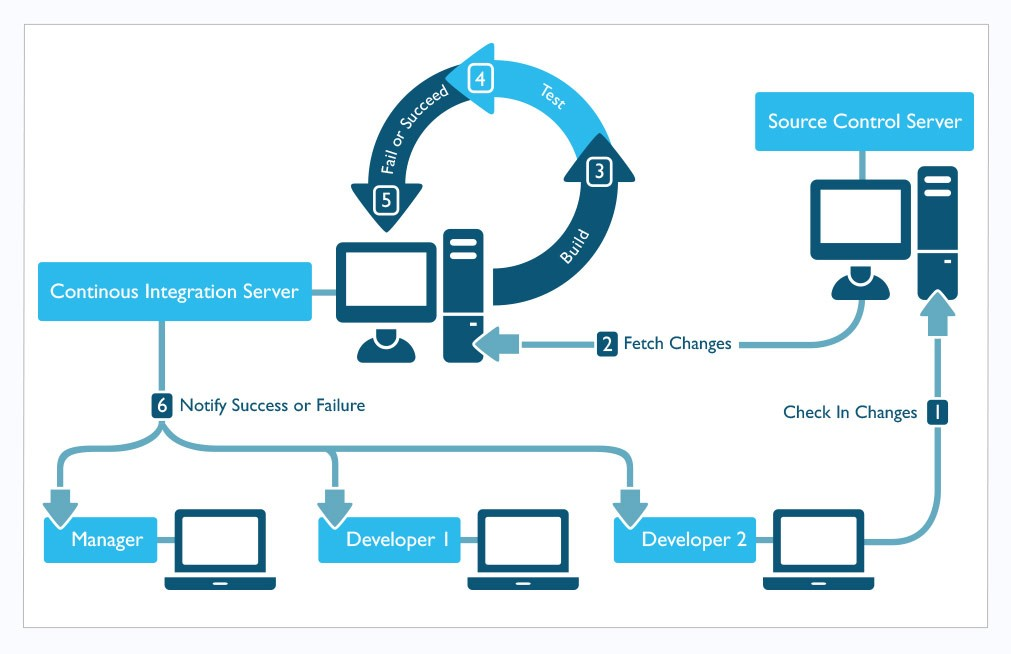
\includegraphics[width=\linewidth]{content/images/continuous_integration}\
	\quelle\url{https://insights.sei.cmu.edu/devops/2015/01/continuous-integration-in-devops-1.html}
	\caption[Continuous Integration]{Continuous Integration\\}
	\label{fig:ContinuousIntegration}  
\end{figure}\noindent 
Wie zu erkennen ist, sorgt ein zentraler "'Continuous Integration Server"' für das Bauen und Testen der Software und informiert die zuständigen Entwickler über den Status. In der Regel wird dies bei jeder Code Änderung durchgeführt, sodass direkt erkannt wird, ob eine Änderung des Codes zu einem Erfolg oder einem Fehlschlag führt.
\\
\begin{quote}
	"'The concept of Continuous Integration (CI) was a first step that significantly sped up the lifecycle of a product, pushing developers to commit/integrate more frequently to a shared repository, triggering automated unit-tests after each commit; as direct consequence, this helped to detect problems richt after a bad commit and reduced the necessity of back-tracking to individuate the issue in changes happend far away in time."'\cite[in Introduction]{IEEE:CDMitJenkins}
\end{quote}
Continuous Delivery ist eine natürliche Erweiterung von Continuous Integration. Trotzdem unterscheiden sich die beiden Begriffe nicht wirklich von einander. Während bei der Continuous Integration wert darauf gelegt wird, Software möglichst Fehlerfrei zu erzeugen, wird bei Continuous Delivery  darauf wert gelegt, Software möglichst regelmäßig zu deployen. Continuous Delivery beinhaltet Continuous Integration und erweitert diese um das ausliefern.

\section{Continuous Delivery Pipeline}
\label{sec:Continuous Delivery Pipeline}
Es wurden bisher die Vorteile von Continuous Delivery erläutert, wie funktioniert jedoch Continuous Delivery im einzelnen? Die einzelnen Schritte werden durch die \textit{Continuous Delivery Pipeline} beschrieben. Dabei wird der Durchlauf der Pipeline automatisch durchgeführt. Die Continuous Delivery Pipeline integriert zum einen
Die Folgende Abbildung zeigt eine mögliche Pipeline. Das Deployen in die Produktionsumgebungen "'PRODBLUE"' und "'PRODGREEN"' muss in diesem Beispiel jedoch manuel, durch klicken auf Trigger, erfolgen.

\begin{figure}[htb]
    \centering 
    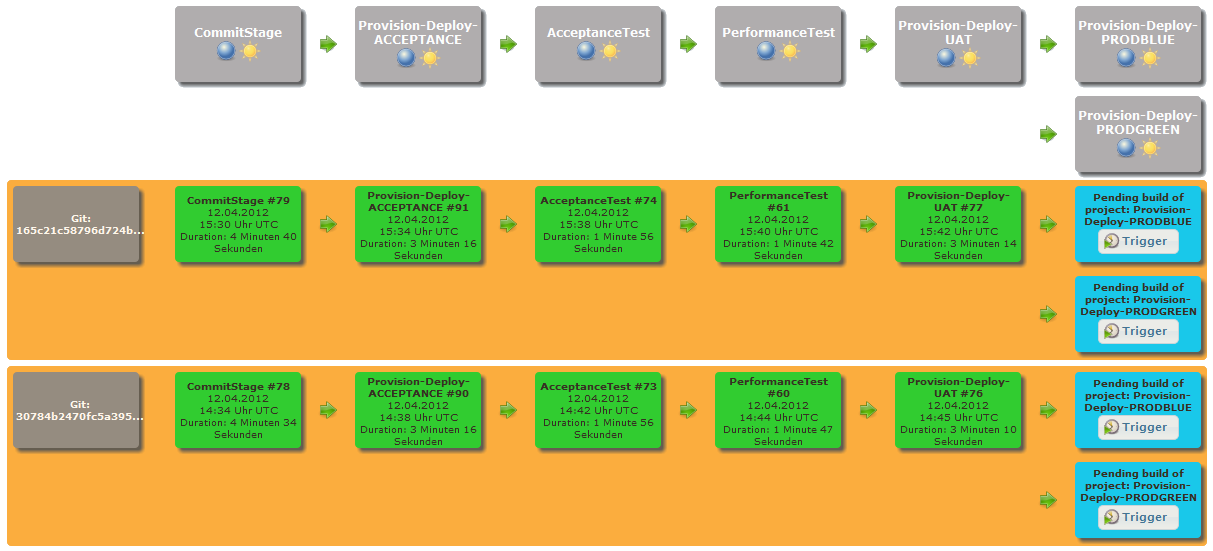
\includegraphics[width=\linewidth]{content/images/pipeline}\
    \quelle\url{https://blog.codecentric.de/en/2012/04/continuous-delivery-in-the-cloud-part1-overview/}
    \caption[Continuous Delivery Pipeline]{Continuous Delivery Pipeline\\}
    \label{fig:ContinuousDeliveryPipeline}  
\end{figure}\noindent 
Wie man in der Abbildung sehen kann beinhaltet die Pipeline alle nötigen schritte, welche zuvor in \nameref{subsec:ContinuousIntegration} besprochen wurden. Hier sei noch einmal erwähnt, dass Continuous Integration alle Prozesse, bis auf den letzten (das Deployment), beinhaltet. Continuous Integration und Delivery unterscheiden sich, wie schon zu vor erwähnt, nur beim letzten Schritt, dem Deployen. Dieser wird jedoch bei Continuous Delivery Manuel ausgeführt. Unter ausgeführt ist hierbei zu verstehen, dass ein Prozess, hier durch einen klick, gestartet wird, welcher die Software, bzw. das Artefakt, automatisch in die Produktion bringt.

\section{Werkzeuge für Continuous Delivery}
\label{sec:WerkzeugeCD}
Es wurde bisher erläutert was Continuous Delivery ist, welches Vorteile es hat und welche Voraussetzungen gegeben sein müssen, damit Continuous Delivery eingeführt werden kann. Es wurde ebenfalls mit Abschnitt \ref{sec:ContinuousIntegration} \nameref{sec:ContinuousIntegration} und Abbildung \ref{fig:ContinuousIntegration} \nameref{fig:ContinuousIntegration} der Begriff \textit{Continuous Integration Server} eingeführt. Es wurde jedoch noch nicht geklärt was dieser Server genau ist und welche konkreten Aufgaben dieser besitzt. Dies soll in diesem Abschnitt geklärt werden. Zudem sollen weitere Werkzeuge vorgestellt werden, der für den \textit{Continuous Delivery Prozess} nützlich sein können. Es soll jedoch nicht die konkrete Funktionsweise von Werkzeugen erläutert werden. Einige Werkzeuge werden zum besseren Verständnis genauer erklärt als andere.
In Abschnitt \ref{sec:ContinuousIntegration} \nameref{sec:ContinuousIntegration} wurde der Begriff "'Continuous Integration Server"' erwähnt, jedoch nicht genauer erläutert. Was es mit diesem Begriff genau auf sich hat, wird nun geklärt. 
\\\\
\subsubsection*{Continous Integration Server: Jenkins}
Der Begriff \textit{Continuous Integration} wurde bereits genau erläutert. Ein \textit{Continuous Delivery Server} ist nichts anderes, als eine Applikation die auf einem Server läuft, welche die nötigen Teilprozesse von \textit{Continuous Integration} ausführt. Wird noch einmal die Abbildung \ref{fig:ContinuousIntegration} \nameref{fig:ContinuousIntegration} betrachtet, ist der Server, auf dem die Applikation läuft, direkt neben der Box, in der "Continuous Integration Server" steht abgebildet. Ein Beispiel "Continuous Integration Server" könnte \textit{Jenkins} sein. \textit{Jenkins} ist ein sogenanntes "'Build and Management"' Werkzeug.

\begin{quote}
	"'Jenkins is an Open Source (OSS) CI Platform, whose initial objective has been the automation of the  and test process. The build system is completely written in Java and is easily extensible thanks to its plugins architecture and to extension points left into its object model. this makes of jenkins a highly customizable and flexible tool, able to cover many possible scenarios and requirements thatnks to thousands of plugins developed by its huge Open Source Community."'\cite{IEEE:CDMitJenkins}
\end{quote}
Ein "'Continuous Integration Server"'  wie \textit{Jenkins} ist die zentrale applikation, wenn es um \textit{Continuous Integration/Delivery} geht.
\begin{quote}
	"'[..] If CI startet as automation of the development phase only, pretty soon the revolution embraced the test-phase of the QA team and the deployment into various envirnment of the Ops team, involving the whole lifecycle of a product and introducing a new concept: Continuous Delivery (CD)"'\cite{IEEE:CDMitJenkins}
\end{quote}
\textit{Jenkins} hat dafür gesorgt, dass \textit{Continuous Delivery} leichter wurde. Mit der Applikation war es nun möglich, in wenigen Schritten eine eigene \textit{Continuous Delivery Pipeline} aufzubauen.

\subsubsection*{Build-Management-Tool}
\textit{Build-Management-Tool}, nicht zu verwechsel mit einem "'Build and Management"' Werkzeug, dient in erster Linie dazu, das bauen einer Software zu standardisieren. Einige bekannte Vertreter für Java sind: Maven, Ant, Gradle. Jeder dieser drei \textit{Build-Management-Tools} arbeitet auf Basis einer zentralen Datei in der die Anweisungen stehen, wie die Software gebaut werden soll. Das beinhaltet unter anderem die nötigen Abhängigkeiten (auch Dependency-Management genannt), sowie die Pfade zu den Dateien, welche zusätzlich eingebunden werden sollen.
\\\\
Durch \textit{Build-Management-Tools} können zudem zusätzliche Aktionen durchgeführt werden, wie zum Beispiel das ausführen von Unit-Tests, sowie die Steuerung darüber, was bei fehlgeschlagenen Tests passieren soll.
\\\\
Unter anderem nutzt \textit{Jenkins} solche \textit{Build-Management-Tools} zum bauen der jeweiligen Projekte.

\subsubsection*{Automatischer Aufbau der Infrastruktur}
Nachdem Werkzeuge eingeführt worden sind, mit deren Hilfe standardisierte Software innerhalb und außerhalb von \textit{Continuous Integration}, gebaut werden kann. Muss, damit \textit{Continuous Delivery} durchgeführt und ebenfalls standardisiert werden kann, eine bzw. zwei neue Werkzeuge eingeführt werden.
\\\\
Damit Software automatisch, im Rahmen von \textit{Continuous Delivery}, ausgeliefert werden kann, muss neben den Tests auch das aufbauen der Infrastruktur automatisiert werden. Zwei Werkzeuge um dies zu erreichen sind \textit{Chef} und \textit{Puppet}.
\begin{quote}
	"'Puppet and Chef are the most commonly used IT Automation Tools used by DevOps to set up the infrastructure, speeding up the process of installing the required software, moddleware and various dependencies."'\cite{IEEE:CDMitJenkins}
\end{quote}
Damit Software ohne Probleme automatisch deployed werden kann, müssen ggf. Änderungen an der Infrastruktur durchgeführt werden bzw. eine neue Infrastruktur aufgesetzt werden. Letzteres ist zum Beispiel bei der Skalierung notwendig. Damit jede Instanz gleich, bzw. jede Änderung der vorhandenen Instanzen nachvollzogen werden kann, müssen alle Schritte dokumentiert werden. Die technische Dokumentation geschieht mit Hilfe von \textit{Chef/Puppet}. Nach dieser Dokumentation kann das jeweilige Werkzeug gestartet werden und eine standardisierte Infrastruktur wird aufgebaut.

\subsection{Versionierung von Artefakte}
Zuletzt muss noch eine Möglichkeit gefunden werden, um die einzelnen Versionen von Artefakten zu Versionieren und sicher zu lagern. Hier sei auf die Werkzeuge \textit{Nexus} bzw. \textit{Artifactory} verwiesen.
\\\\
Beide werkzeuge

\section{Einführung von Continuous Delivery}
\label{sec:EinfuehrungCD}
In Kapitel \ref{sec:problemstellung} \nameref{sec:problemstellung} wurde bereits ein Fall beschrieben, in der kein Continuous Delivery eingesetzt wird. Darauf aufbauend wird nun Schritt für Schritt die vorhandene Softwareentwicklung in Continuous Delivery überführt.
\\\\
Damit das Dependencie Management und automatisieren von Tests bzw. das ausführen zusätzlicher Aktionen erleichtert wird, wird zunächst ein Build-Management-Tool eingeführt. Dadurch wird sichergestellt, dass Software idempotent gebaut werden kann. Der Build-Prozess ist dadurch Standardisiert und kann beliebig oft wiederholt werden.
\\\\
Wie bereits erläutert wurde, ist in diesem Beispiel die Qualitätssicherung zwar ein Teil der Softwareentwicklung, jegliche Tests werden jedoch nur manuell ausgeführt, was zu regelmäßigen, unentdeckten Fehlern führt. Daher muss zunächst einmal dafür gesorgt werden, dass Unit-Tests geschrieben werden, welche vor dem Bauen der Software, die Code Qualität und Richtigkeit überprüft.  Test-Driven-Development (TDD)\footnote{TDD wird hier nur erwähnt und nicht weiter erläutert. Es sei auf Fachliteratur zu diesem Thema verwiesen.} ist einer der Möglichkeiten, sicherzustellen, dass Tests regelmäßig geschrieben werden. Zusammen mit dem eingeführten Build-Management-Tool können nun, vor dem Bauen der Software, die Unit Tests durchlaufen und dadurch der Code der Software überprüft werden.
\\\\
Nun ist zu mindestens Sichergestellt, dass diese Art der Tests automatisiert ablaufen und nicht mehr manuell durchgeführt werden müssen. Jedoch müssen noch Akzeptanz-, Performanz- und Integrations-Tests automatisiert werden. Diese Tests können jedoch nicht immer durch das Build-Management-Tool abgedeckt werden. Daher Wird nun ein "'Build and Management"' Werkzeug wie Jenkins\footnote{siehe: https://jenkins.io/} eingesetzt wird, welches sowohl die Software baut, unter anderem mit dem eingeführten Build-Management-Tool, als auch die anderen Tests abbilden kann. Wie die Software genau funktioniert, soll hier jedoch nicht weiter erläutert werden. Es sei nur erwähnt, dass es durch Konfiguration und Plugins möglich ist, die oben genannten Tests innerhalb von Jenkins abzubilden. Es wurde eine \textit{Continuous Delivery Pipeline} erschaffen. Die Abbildung \ref{fig:ContinuousDeliveryPipeline} \nameref{fig:ContinuousDeliveryPipeline} zeigt ein ausschnitt aus dem "'Build and Management"' Werkzeug Jenkins. Außerdem ist es durch Jenkins möglich jeden Schritt zu Überwachen und zu Protokollieren, sowie nach jedem Schritt zu stoppen, sollte ein Fehler auftreten. Dadurch ist es möglich frühzeitig Fehler zu erkennen und diese zu beheben.
\\\\
Es wurde nun dafür gesorgt, dass sowohl das Bauen, als auch jegliche Tests automatisiert wurde. Dadurch kann die Software Standardisiert gebaut und getestet werden. Durch die Automatisierung ist es zusätzlich möglich die \gls{glos:TTM} Zeitspanne deutlich zu kürzen, da automatisch durchgeführten Tests, meistens kürzer und genauer sind, als wenn man diese manuell ausgeführt hätte. Außerdem werden unter anderem dadurch Fehler frühzeitig erkannt und können behoben werden, bevor die Software in Produktion geht. Durch die durchgeführten Änderungen am Entwicklungsprozess, ist es nun möglich bei jeder Änderung des Quellcodes, die Software standardisiert zu bauen und zu Testen. Dadurch erhält der, bzw. die Entwickler regelmäßig und in kurzen Abständen eine Rückmeldung, ob die durchgeführten Änderungen am Code zu Problemen führen oder die Software weiterhin funktioniert. Dies führt dazu, dass regelmäßig releasefähige Software erzeugt wird, welche in Produktion gebracht werden kann.

% siehe: https://stackoverflow.com/questions/28608015/continuous-integration-vs-continuous-delivery-vs-continuous-deployment
\chapter{Zusammenfassung und Ausblick}
\label{chap:zusammenfassungUndAusblick}

\section{Zusammenfassung}
\label{sec:zusammenfassung}
Continuous Delivery ist ein großes Thema. Dies sieht man an der zuvor genannten \nameref{sec:problemstellung}. Es wurde ein konkretes Beispiel genannt und dessen Probleme herausgearbeitet. Danach wurden die Leitfragen dieser Ausarbeitung geklärt. Als erstes sollte geklärt werden, was "`Continuous Delivery"' ist. Danach wurde der Begriff "`Continuous Delivery Pipeline"' eingeführt und darauf aufbauend der Entwicklungsprozess, des in der Problemstellung genannten Beispiels, in Continuous Delivery überführt.
\\\\
Zunächst wurde jedoch eine Systematische Literaturrecherche durchgeführt. Dafür wurden Inhaltliche Auswahl- und Ausschlusskriterien aufgestellt. Danach wurde mit Hilfe des PICOC-Ansatzes zunächst die Begriffe und der Personenkreis für die eigentliche Suche ermittelt. Außerdem wurden zusätzliche Anmerkungen zur Recherche, bezogen auf diese Ausarbeitung,  getroffen. Es wurden die eigentlichen Suchstrings gebaut und die zu durchsuchenden Quellen eingeführt. Darauf aufbauend wurden die Ergebnisse der Recherche wiedergegeben (Das Rechercheprotokoll ist im Anhang zu finden). Es stellte sich heraus, dass "`Google Scholar"' zwar viele Ergebnisse liefert, jedoch nicht viele relevante. Außerdem ist anzumerken, dass die wenigen Relevanten Ergebnisse der "`Google Scholar"'-Suche auf IEEExplore Dokumente verweisen, welche bereits bei der suche in dem genannten Archiv gefunden worden sind und daher nicht weiter betrachtet wurden. Die Ergebnisse der Systematischen Literaturrecherche wurden zwar Berücksichtigt und durchgelesen, jedoch umfassten sie im nach hinein betrachtet zu weitgehende Informationen, sodass sie nicht zum erläutern der Grundlagen dienen konnten und nur die im Literaturverzeichnis angegebenen Quellen verwendet wurden.
\\\\
Aufbauend auf die Systematische Literaturrecherche wurde das Thema "`Continuous Delivery"' behandelt. Dafür wurde zunächst der Begriff "`Continuous Delivery"' erläutert und es kristallisierte sich heraus, dass Continuous Integration ein großer Bestandteil von "`Continuous Delivery"' ist. Daher wurde zunächst Continuous Integration erläutert und die Teilprozesse kurz erwähnt. Darauf aufbauend wurde die "`Continuous Delivery Pipeline"' eingeführt und mit Hilfe von Continuous Integration und Delivery erläutert. Mit Hilfe der Pipeline wurde anschließend das Beispiel aus der Problemstellung um Continuous Delivery erweitert.
\\\\
Zuletzt erfolgt nun eine kritische Reflektion des Themas und ein Ausblick.

\section{Kritische Reflektion}
\label{sec:kritischeRelfektion}
Continuous Delivery ist ein Großes und für Unternehmen interessantes Thema. Es kann dafür sorgen, dass die Zeitspanne von der Idee bis zur Produktion (die Time-to-Market (TTM) Zeitspanne) verkürzt wird. Dadurch können Unternehmen sehr viel Geld sparen und Umsetzungen viel schneller in die Produktion bringen. Zusätzlich kann man den Build- und die Test-Prozesse durch Continuous Delivery standardisieren und automatisieren. Durch standardisierte Tests kann sichergestellt werden, dass auch nach Änderung einer Software, die Funktionalitäten weiterhin funktionieren. Außerdem bekommen Entwickler dadurch eine schnelle Rückmeldung über den Status der Software. Sie können direkt sehen, ob die Software ohne Fehler gebaut werden konnte und alle Tests erfolgreich durchgelaufen sind oder ob Fehler aufgetreten sind. Durch Automatisierte Tests kann außerdem sichergestellt werden, dass die Fehler in Produktion deutlich verringert werden, da die gleichen Tests ausgeführt werden können, welche vor einer Änderung erfolgreich ausgeführt wurden. Zudem kann der Prozess beliebig oft mit dem gleichen Einstellungen durchlaufen werden und das gleiche Ergebnis erwarten. Der Prozess ist also Idempotent.
\\\\
Jedoch muss \textit{Continuous Delivery} auch kritisch betrachtet werden. Zum einen sind nicht alle Tests automatisierbar. Zum Beispiel ist ein Oberflächentest sehr schwer automatisierbar. Zum anderen kann es schwer sein ein bestehenden Entwicklungsprozess um Continuous zu erweitern. Zusätzlich werden dafür ggf. neue Werkzeuge wie ein "`Build-management-Tool"' oder einen sogenannten Continuous Integration Server wie Jenkins benötigt. Entwickler müssen sich zunächst einmal mit diesen Werkzeugen auseinander setzten und erlernen. Manch ein Werkzeug ist recht teuer und durch das fehlende Wissen, kann es schnell passieren, dass falsche oder zu teure Software gekauft wird. Möchte ein Unternehmen also Continuous Delivery einführen, hat jedoch selber keine Ahnung des Themas, ist es ratsam einen Experten dazu zu holen, der einen beraten kann und ggf. Schulungen durchführen kann. Weiter sollten möglichst alle, aber auf jeden Fall ein Großteil der Entwickler davon überzeugt sein oder überzeugt werden können eine Veränderung des Entwicklungsprozesse zuzulassen bzw. durchzuführen.
\\\\
Es sei hier noch erwähnt, dass der Vergleich zwischen Continuous Integration vs Delivery vs Deployment ausgelassen wurde, da diese Begriffe nicht eindeutig definiert sind und zum Teil synonym zueinander verwendet werden. Es gibt keine direkten Vergleiche außerhalb von Blogs, jedoch wird für jeden klar, der sich mehr mit diesem Thema beschäftigt, das zum Teil die Übergänge fließend sind. Hier sollte sich jeder ein eigens Bild machen und sich selber mit dem Thema beschäftigen.

\section{Ausblick}
\label{sec:ausblick}
Continuous Delivery ist, wie bereits erwähnt, ein Großes Thema, daher konnte in dieser Ausarbeitung nur eine kleine Einführung des Themas stattfinden. Es kann jedoch noch zusätzlich Continuous Integration, Delivery und Deployment verglichen werden und die Werkzeuge erläutert werden, die zum Umsetzten des jeweiligen Prozesses benötigt werden. Man kann auf verschiedene Teilgebiete von Continuous Delivery, wie zum Beispiel dem "`Build-management-Tool"' eingegangen werden. Genauso kann man auf das "`Build und Management"' Werkzeug Jenkins eingegangen werden.
\\\\
Außerdem ist es möglich auf die Unterschiede in der Time-to-Market Zeitspanne zwischen einem Entwicklungsprozess ohne Continous Delivery und einen mit Continous Delivery einzugehen und darauf aufbauend die Kosten der jeweiligen Prozesse zu vergleichen.


% ***************************** BIBLIOGRAPHY **********************************
\baselineskip=14pt
\addcontentsline{toc}{chapter}{\protect\numberline{}\bibname}
\bibliography{bib/thesis}

% ******************************* APPENDIX ************************************
\appendix
\baselineskip=18pt
\chapter{Anhang}
\label{chap:anhang}

%Befehle für Glossar
\newglossaryentry{glos:TTM}{
    name=Time-to-Market,
    description={Unter dem Begriff Time-to-Market wird die Zeit von der Produktentwicklung bis zur Auslieferung auf dem Markt verstanden. In dieser Zeit müssen Kosten für die Erstellung/Entwicklung aufgebracht werden, es spielt aber keine Umsätze ein. Daher strebt jedes Unternehmen eine möglichst geringe Time-to-Market Zeit an. Insbesondere wenn es um Wettbewerb geht, muss diese Zeit kurz gehalten werden.}
}

\section{Rechercheprotokoll}
\label{sec:rechercheprotokoll}



\end{document}
